\chapter{Plans}\label{C:con}

\section{Proposal Review}

\subsection{Stage 1} 
This will primarily be research into the problem itself.This includes the physical
science behind it and the algorithms mentioned above. While a portion of this will be
continuous throughout the project the bulk should be completed by 22 April with a
presentation given to GNS around this time.
\\\\
Completed but presentation has yet to be given but will be arranged at a time convenient to GNS.

\subsection{Stage 2} 
Each of the above techniques will then be further investigated to determine their fit for the proposed problem. This is to remove any redundancy and avoid complication during stage 3. This should be completed by 10 May with the completion of a one page report.
\\\\
Completed - work can be found within background section.

\subsection{Stage 3} 
The third task will be determining the evaluation methods used to benchmark the
success of each technique. A fitness function for the given problem will be determined
using the pre-existing work and communication with a geotech at GNS. This should
be completed by 19 July by GNS acceptance of the documented methods.
\\\\
This has changed as the fitness function will be the same as that found within Aaron's work. However the collection of benchmark data from Aaron's work has commenced. This will be completed by the 21st of June.

\subsection{Stage 4} 
The techniques that meet the problems criteria will then be developed in Java and
tested against existing benchmarks/standards a number of times to ensure statistical
confidence. These results will be collated into an appendix by 8 September, this will
be attached to the final report.
\\\\
The implementation of these techniques will be completed by 15 July.

\subsection{Stage 5} 
The evaluation techniques that were developed during stage 3 will then be tested
against the remaining algorithms and the existing parallel linear genetic programming
solution. Again these tests will be run multiple times to ensure statistical confidence
and be written into an appendix by 27 September.



\subsection{Stage 6} 
The final stage will be to ensure all the resources used and developed during the
project are in a presentable format. This includes a written report, oral presentation
and a tidy code repository for any future work.
\\\\
Written Report - 18 October
\\
Oral Presentation - 16 November
\\
Tidy Code Repository - 16 November

\section{Gantt Chart}

\begin{figure}[h]
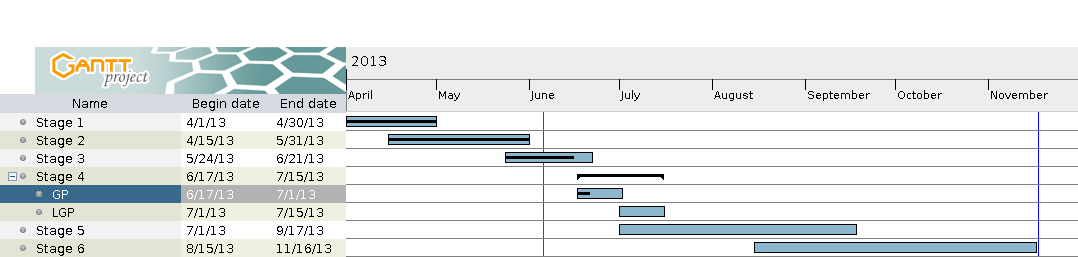
\includegraphics[width=170mm]{ganttV1.png}
\caption{Gantt Chart Created 3 June 2013}
\end{figure}

\section{AI Libraries}
Rather than reinventing the wheel there already exist a number of Java libraries built specifically for the implementation of genetic programming programs. Within Victoria University there has been a substantial amount of work done using the ECJ library. Due to this background and the amount of documentation available this will be used in the creation of the GP. There are currently no open source Java LGP libraries. Slash-A is the only out of the box LGP supporting library that has been developed and released but this is written in C++ and creating a new libCPS wrapper would be redundant. Carlton Downey has produced a Java LGP but it is currently not in the public domain. If this software cannot be obtained a LGP library will be built specifically for this research.